\subsection{Project Management}

\noindent{}Our project management strategy is based on the Agile methodology.
This allowed us to adapt to the changing requirements of the project
efficiently. We have divided the work into sprints, each focusing on specific
aspects of the project.

\begin{figure}[h]
    \centering{
    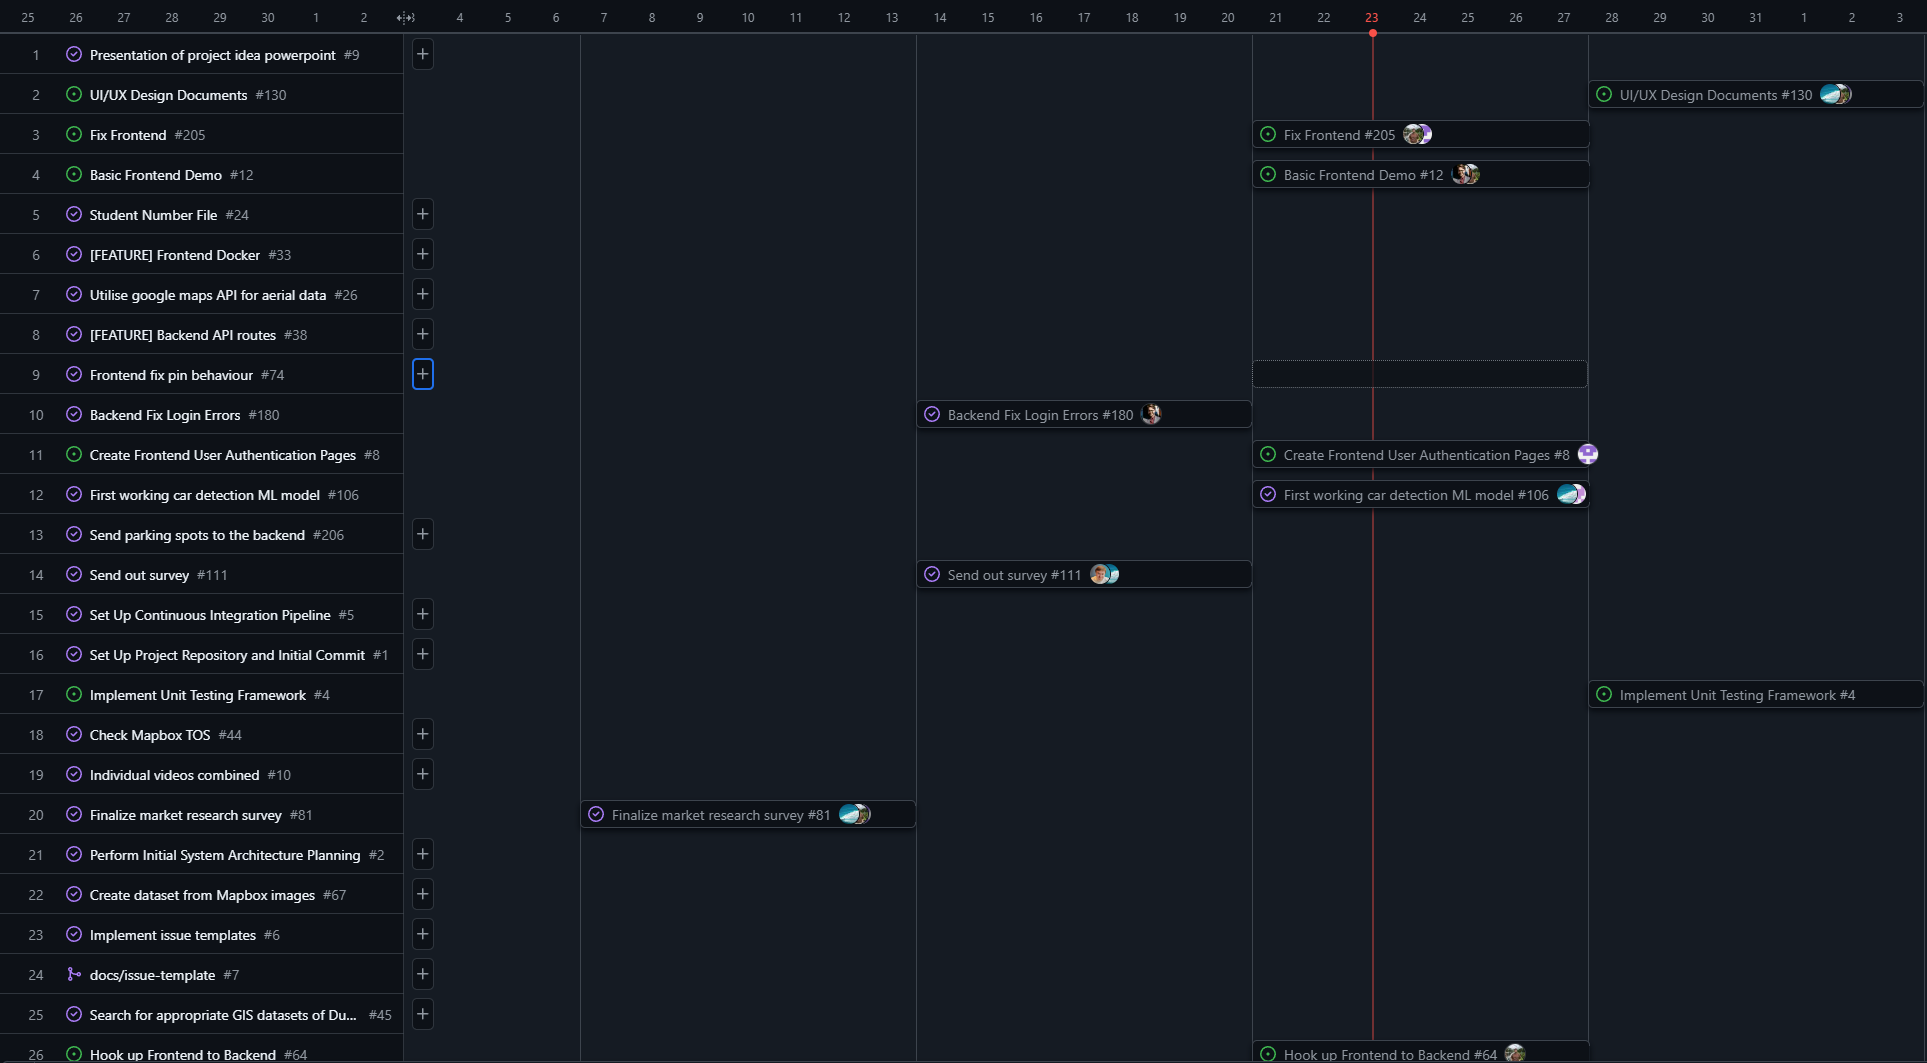
\includegraphics[width=0.95\columnwidth]{images/gantt.png}
    \caption{Section of our Gantt Chart}
    \label{fig:gantt}
  }
\end{figure}

% Adds page break to ensure blocking
\pagebreak{}

\noindent{}Daily stand-ups help maintain accountability and ensure that each
team member is aligned with the the tasks at hand that week. We are also
leveraging \textit{GitHub Projects} to track progress, set milestones and
delegate tasks efficiently across the team. We regularly perform retrospectives
to reflect on the previous weeks work and identify anything that needs to be
improved for the next week. We also perform weekly sprint planning sessions to
assign goals for that particular week, and to ensure that workload is spread
evenly across the team. Collaboration between team members is facilitated
through a \textit{Discord} server, where we can communicate and share resources.
We have setup individual channels for each section of the team to discuss
relevant topics, and remain in touch in case of issues or queries.

\begin{figure}[h]
    \centering{
    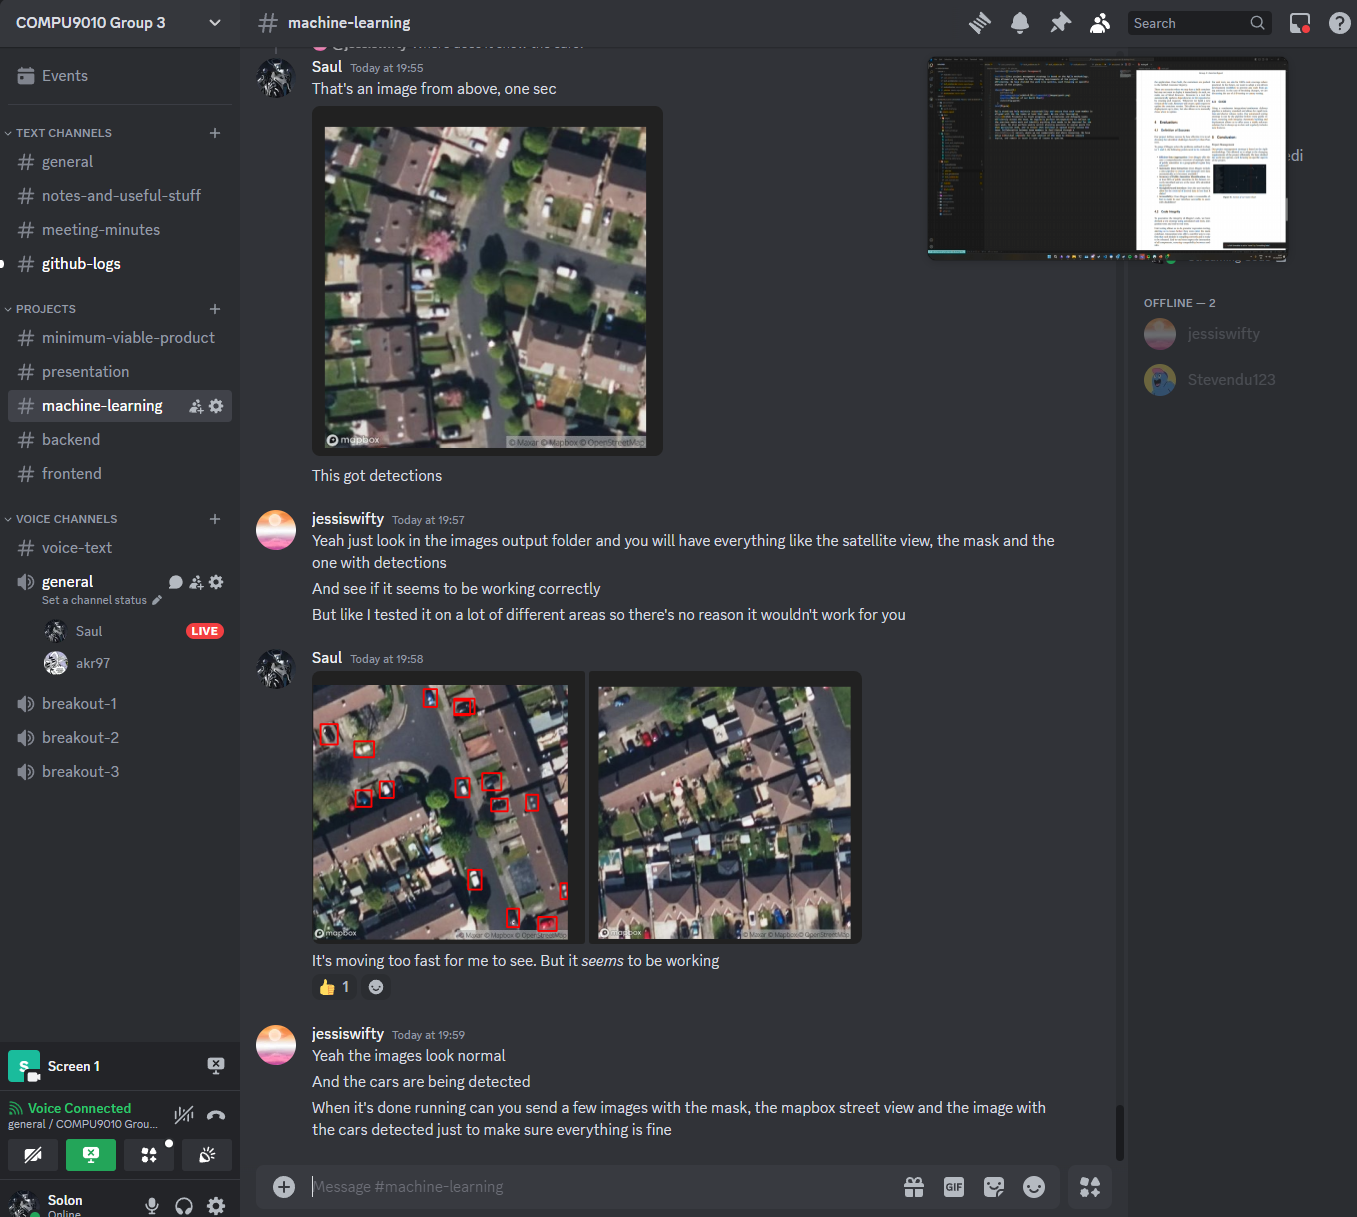
\includegraphics[width=0.95\columnwidth]{images/discord.png}
    \caption{Example of our Discord Server}
    \label{fig:discord}
  }
\end{figure}

\subsection{Current Challenges}

\noindent{}The biggest challenges we currently face include:
\vspace{-3mm}
\begin{itemize}
  \item{Ensuring detection accuracy}
  \item{Implementing additional data sources}
  \item{Improving data-pipeline}
\end{itemize}
\vspace{-3mm}

\noindent{}The current parking detection model has (in certain cases) a
propensity to misclassify some residential chimneys as parking spots. This is
due to multiple issues, for example- our satellite imagery is only precise to
20cm, and at times, the image quality is too low to distinguish the shapes. We
believe this is solvable by using masks or additional heuristics to subtract
those misclassification from the overall dataset.

\noindent{}Notably, as \textit{Magpie} is a project with low amounts of funding.
We cannot acquire higher quality data, if \textit{Magpie} were to scale, we
could also purchase satellite imagery with higher resolution. This would likely
provide enough of a difference between parking spots and chimneys to prevent
misclassification.

\noindent{}As mentioned in section 2.1, we decided to focus on parking detection
initially, as it both sets us apart from other tools, and is information that is
not easily accessible. However, a single data source would not be sufficient to meet
our goals. As such, implementing additional data sources is crucial to the overall
success of the project.

\noindent{}Early on in the project, we decided to use a \textit{Batch} process
when loading our data. We decided to take this approach for three reasons:
\vspace{-3mm}
\begin{itemize}
  \item{Reduces access required to the cluster database}
  \item{Allowed for manual checking of data before upload}
  \item{Reduced the amount of backend work}
\end{itemize}
\vspace{-3mm}

\noindent{}While none of these reasons are no longer relevant, uploading a Batch
currently requires Saul (provider of our cluster) to manually run, validate and
upload the data. While likely sustainable, this is not the \textit{best}
solution. Further investigation is needed to determine the best way of
automating this task.

\noindent{}\textbf{Plan for remaining time} To achieve a successful outcome
within the remaining timeframe, we will focus on several key priorities. 
\begin{itemize}
    \item{Firstly, we will work on optimising our parking detection model to
    enhance it's detection accuracy.}
    \\

    \item{Secondly, we will focus on implementing additional data sources. This
    will improve the overall utility of the application and provide a more
    comprehensive picture to users of avalible public amenities.}
    \\

    \item{Finally, we will work on improving the overall quality of our project.
    This will take many forms, from improving our documentation, tests, and
    code. To ensuring that \textit{Magpie} is a robust and reliable tool for our
    users.}
    \\
\end{itemize}
\vspace{-3mm}

\subsection{Conclusion}
In conclusion, \textit{Magpie} is a project that aims to provide Urban Planners
a tool that allows them to access and analyse data in a single, easy to use,
platform. To date we have achieved a number of key milestones, and provided a
minimum viable product that can be expanded to achieve our project goals.
\\ % My hatred for the necessity of this is infinite, however otherwise the formatting is off
\\
\\
\\
\\
\\
\\

% Adds page break to ensure blocking
\pagebreak{}